\documentclass{beamer} % optional mode: handout, notes

\usepackage[english]{babel}
\usepackage[T1]{fontenc}
\usepackage[utf8]{inputenc}

\usepackage{algorithm}
\usepackage{algorithmic}
\usepackage{amsmath}
\usepackage{amssymb}
\usepackage{graphicx}
\usepackage{lmodern}
\usepackage[numbers]{natbib}
\usepackage{physics}
\usepackage{xurl}

\newcommand{\myQuote}[1]{``#1''}

\definecolor{matnat}{RGB}{0,130,198}
\setbeamercolor{footlinecolor}{bg=white, fg=matnat}
\setbeamercolor{title}{fg=blue}
\setbeamercolor{subtitle}{fg=matnat}

\setbeamertemplate{footline}{
	\leavevmode
	\hbox{
		\begin{beamercolorbox}[wd=.1\paperwidth,ht=10.25ex,dp=1ex,center]{footlinecolor}
			\hspace*{0.4cm } 
\includegraphics[scale=0.1]{media/siegel.jpg}
		\end{beamercolorbox}

		\begin{beamercolorbox}[wd=0.6\paperwidth,ht=10.25ex,dp=1ex,center]{footlinecolor}
			\parbox{\paperwidth}{\hspace*{.5cm}\textcolor{matnat}{\inserttitle \hspace*{2cm} \insertsection}  \\[0.13cm] \hspace*{0.44 cm} \textcolor{matnat}{\insertshortauthor} \vspace{0.8cm} }
		\end{beamercolorbox}

		\begin{beamercolorbox}[wd=.3\paperwidth,ht=10.25ex,dp=1ex,right]{footlinecolor}
			
\includegraphics[scale=0.4]{media/uni.jpg} \hspace*{1cm}
		\end{beamercolorbox}
	}
}

\title{Bayesian Inference}
\author{Oliver Filla}
\date{November 20, 2024}

\begin{document}
	\frame{\titlepage}
	\frame{\tableofcontents}

	\section{Probability}
	\subsection{Determinism and its Limits}
	\begin{frame}{Determinism and its Limits}{Why do we need Probabilities?}
		\only<2->{\large Determinism}
		\begin{itemize}
			\item<2-> \emph{Every event is determined by past events.}
			\item<3-> assumed in Classical Mechanics
								\note<3>{If we know the initial conditions, we can predict the future perfectly.}
			\item<4-> contradicted in Quantum Mechanics?
		\end{itemize}
		\vspace{6pt}
		\only<5->{\large Reality}
		\begin{itemize}
			\item<5-> limited knowledge, e.g. friction
			\item<6-> limited control over initial state, e.g. in chaotic systems
		\end{itemize}
		\vspace{6pt}
		\only<7->{\emph{Example: Throwing dice:} Initial angle and velocity are unknown or difficult to control. It is unknown if the dice are fair.}
		\vspace{6pt}

		\only<8->{$\Rightarrow$ Thus, we need probabilities to predict events!}
		\note{cf. previous talk: probabilies are used to predict!}
	\end{frame}

	\subsection{Frequentist statistics}
	\begin{frame}{Frequentist statistics}
		\note<1>{One way to look at statistics, it's the default view in physics.}
		\only<2->{
			\emph{Probabilities are determined by distributions of random events.}

			They are characterized by the frequency of occurring events.
			\vspace{3pt}
		}

		\only<3->{
			\begin{table}
				\begin{tabular}{l||c|c|c|c|c|c||c}
						& $1$ & $2$ & $3$ & $4$ & $5$  & $6$ & $\sum$ \\
					\hline
					frequency
						&$10$ & $5$ & $7$ & $6$ & $9$ & $7$ & $44$ \\
					probability $[\%]$
						& $23$ & $11$ & $16$ & $14$ & $20$ & $16$ & $100$
				\end{tabular}
		
				\vspace{3pt}
				results of dice rolls; expected PMF $p(i)=1/6=16.\bar 6\,\%$
			\end{table}
		}

		\begin{itemize}
			\item<4-> Probability Mass Function (PMF) (discrete)
			\item<5-> Probability Density Function (PDF) (continuous)
						\note<5>{example: bell curve}
			\item<6-> Cumulative Distribution Function (CDF) (integrated PDF)
		\end{itemize}
		\vspace{3pt}

		\only<7->{$p(6)=\frac{1}{6} \Rightarrow$ \emph{I expect that every 6th dice roll shows a 6, on average.}}
	\end{frame}

	\subsection{Bayesian statistics}
	\begin{frame}{Bayesian statistics}
		\only<2->{\emph{Bayesian statistics describes the credibility of hypotheses.}}

		\vspace{6pt}
		\begin{itemize}
			\item<3-> hypothesis $H$: falsifiable assumption that a specific statement is true,
						e.g. \emph{it will rain today.}
			\item<4-> credibility $C(H)\in[0,1]$: strength of belief in $H$
						\note<4>{Assign a number: $1$ is fully believed, $0$ is fully denied}
			\item<5-> mathematically, credibilities and probabilities are identical
			\item<5-> difference is conceptual
			\item<6> $C(H)$ can be updated with new data
						\note<6>{example: Weather prediction\\}
						 \note<6>{prior: I don't know $\Rightarrow 50\%$ rain\\}
						 \note<6>{see dark clouds\\}
						\note<6>{posterior: $80\%$ rain}
		\end{itemize}
		\vspace{6pt}

		\only<7->{$p(6)=\frac{1}{6} \Rightarrow$ \emph{I believe the hypothesis $H$ \myQuote{the die roll shows a 6} with a credibility of $C(H)=\frac{1}{6}$.}}
	\end{frame}

	\section{Conditional Probability}
	\begin{frame}{Conditional Probability}
		\only<2->{
			\emph{$P(A|B)$ describes the probability of event $A$ with the assumption that event $B$ takes place.}
			\vspace{6pt}
		}
		\begin{columns}[T]
			\begin{column}{0.6\textwidth}
				\begin{itemize}
					\item<3-> read: $P(A \text{ given that } B)$
					\item<4-> filters sets of possible events
					\item<5-> joint probability: both $A$ and $B$:
								$P(A\cap B) = P(A)P(B|A)$
					\item[$\Rightarrow$]<6->
								only when $A$ and $B$ independent:
								$P(A\cap B) = P(A)P(B)$
					\item<7-> joint probability: any $A$ or $B$:
								\only<8->{$P(A\cup B) = P(A) + P(B) - P(A\cap B)$}
					\item[$\Rightarrow$]<9->
								$A$ and $B$ mutually exclusive:
								$P(A\cup B) = P(A) + P(B)$
				\end{itemize}
			\end{column}
			\begin{column}{0.4\textwidth}
				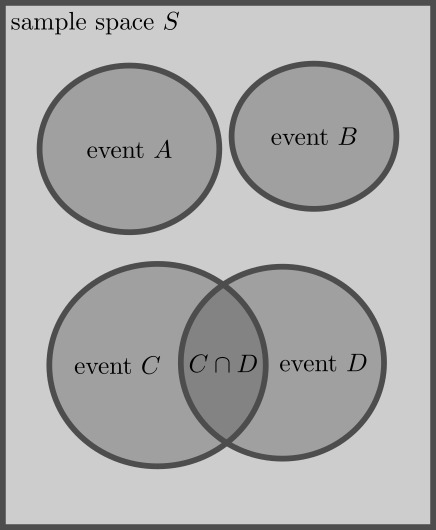
\includegraphics[width=\textwidth]{media/sample_space.jpg}<8->
			\end{column}
		\end{columns}
	\end{frame}

	\subsection{Probability \& Likelihood}
	\begin{frame}{Probability \& Likelihood}
		\only{
			Recap from the talk \emph{The Maximum Likelihood Principle} by~\textsc{Maja~Korbmacher}.
			\vspace{6pt}
		}<1->
		\begin{itemize}
			\item[$\bullet$]<2-> Probability $P$: tool for prediction of events
			\item[$\bullet$]<2-> Likelihood $L$: tool for modelling
			\item[$\bullet$]<2-> equal for given hypothesis $H$ and events $E$
			\item<3-> but only if no prior knowledge is available
			\item<3-> Bayes' theorem generalizes this, using prior knowledge
		\end{itemize}
		\begin{eqnarray}
			\alt<3>{L(H|E) &\overset{?}{=}& P(E|H)}{
				\alt<2>{L(H|E) &=& P(E|H) \nonumber}{\nonumber}
			}
		\end{eqnarray}
	\end{frame}

	\subsection{Bayes' Theorem}
	\begin{frame}{Bayes' Theorem}
		\emph{Bayes' theorem describes the procedure of updating a hypothesis $H$, given that new evidence $E$ is available. It is the scientific method of changing beliefs.}
		\vspace{6pt}
		\begin{itemize}
			\item<2-> Hypothesis $H$
			\item<2-> Evidence $E$
			\item<3-> follows from joint probability $P(E\cap H)$
			\item<4-> overall likelihood $P(E)$ (\emph{law of total probability})
		\end{itemize}
		\begin{eqnarray}
			\alt<5->{
				\only<5->{P_2(H|E) &=& \frac{P(E|H)P_1(H)}{P(E)}}
				\only<6->{\\ \Rightarrow L(H|E) &=& P(E|H) \cdot \frac{P(H)}{P(E)}}
				\only<7>{\\ P(E) &=& P(E|H)P(H) + P(E|\neg H)P(\neg H)}
			}{\nonumber}
		\end{eqnarray}
	\end{frame}

	\begin{frame}{Bayes' Theorem}{Geometric Interpretation}
		\centering
		\begin{columns}
			\begin{column}{0.4\textwidth}
				\begin{itemize}
					\item<2-> square: probability $1$
					\item<3-> prior $P_1(H)$
				\end{itemize}
				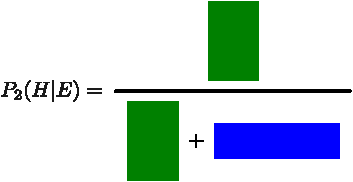
\includegraphics[width=0.9\textwidth]{media/Bayes_geometric_formula}<4>
			\end{column}
			\begin{column}{0.6\textwidth}
				\alt<4>{
					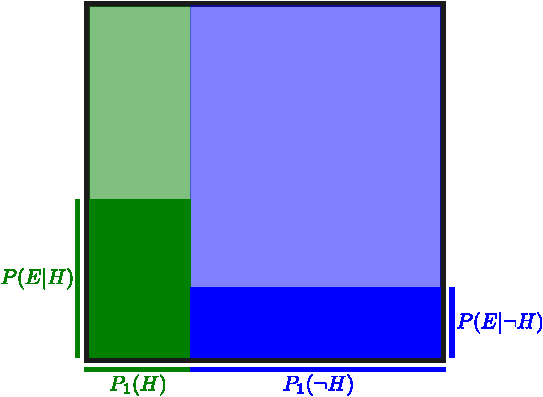
\includegraphics[width=\textwidth]{media/Bayes_geometric.pdf}
				}{
					\alt<3>{
						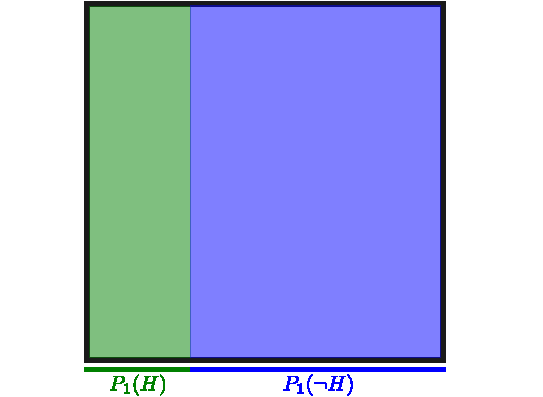
\includegraphics[width=\textwidth]{media/Bayes_geometric_without_data.pdf}
					}{
						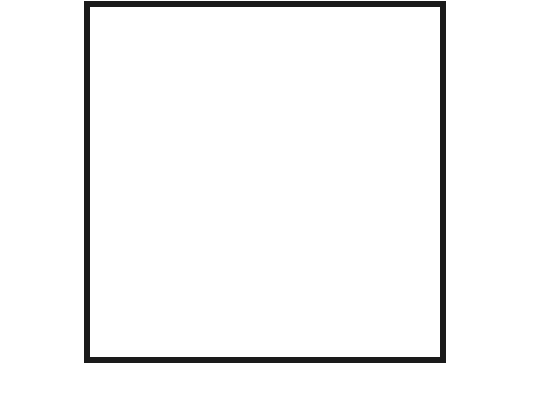
\includegraphics[width=\textwidth]{media/Bayes_geometric_empty.pdf}<2>
					}
				}
			\end{column}
		\end{columns}
		\only<2->{The black square with side length $1$ contains all probabilities.}
	\end{frame}

	\section{Hypothesis Testing}

	\subsection{Updating Credibilities}
	\begin{frame}{Updating Credibilities}{with Bayes' Theorem}
		\begin{eqnarray}
			P_2(H|E) &=& \frac{P(E|H)P_1(H)}{P(E)} \nonumber
		\end{eqnarray}
		\vspace{12pt}

		\only<2->{How to update the credibility of a hypothesis $H$:}

		\begin{enumerate}
			\item<3-> assert prior $P_1(H)$
			\item<4-> evaluate evidence $E$: $\rightarrow$ likelihood $P(E|H)$
			\item<5-> calculate overall likelihood $P(E)$
			\item<6-> calculate posterior probability $P_2(H|E)$
		\end{enumerate}
	\end{frame}

	\subsection{The Posterior Odds ratio}
	\begin{frame}{Updating Credibilities}{The Posterior Odds ratio}
		\only<5->{
			The Posterior Odds ratio compares the posterior probabilities $P_2$ for two different hypotheses $H_{A,B}$.
			\vspace{6pt}
		}
		\begin{itemize}
			\item<2-> relative probability: compare probabilities
			\item<2-> absolute probabilities have limited use
			\item[$\rightarrow$]<3-> $\frac{P(A)}{P(B)}=\frac{1}{2}$ tells event $B$ occurs twice as often
						as event $A$, \\
						\only<4->{for e.g. $P(A)=0.1, P(B)=0.2$ or $P(A)=0.3, P(B)=0.6$.}
			\item<6-> overall likelihood $P(E)$ becomes irrelevant
		\end{itemize}

		\begin{eqnarray}
			\alt<6->{
					\frac{P_2(H_A|E)}{P_2(H_B|E)} &=&
						\frac{P(E|H_A)}{P(E|H_B)}
						\frac{P_1(H_A)}{P_1(H_B)}
				}{\nonumber}
		\end{eqnarray}
	\end{frame}

	\begin{frame}{Example}{rapid antigen tests}
		Assume a \emph{COVID rapid test}
		\only<2->{with a sensitivity of $80\%$, causing $20\,\%$ false-negative results,}
		\only<3->{and a specificity of $98\%$, causing $2\%$ false-positive results.}

		\alt<-3,5->{}{\vspace{12pt} My rapid test is positive: How likely do I have COVID?}
		\note<4>{The likelihood depends on the amount of ill people: If a small amount of people is infected, it is likely that the test is false-positive.}

		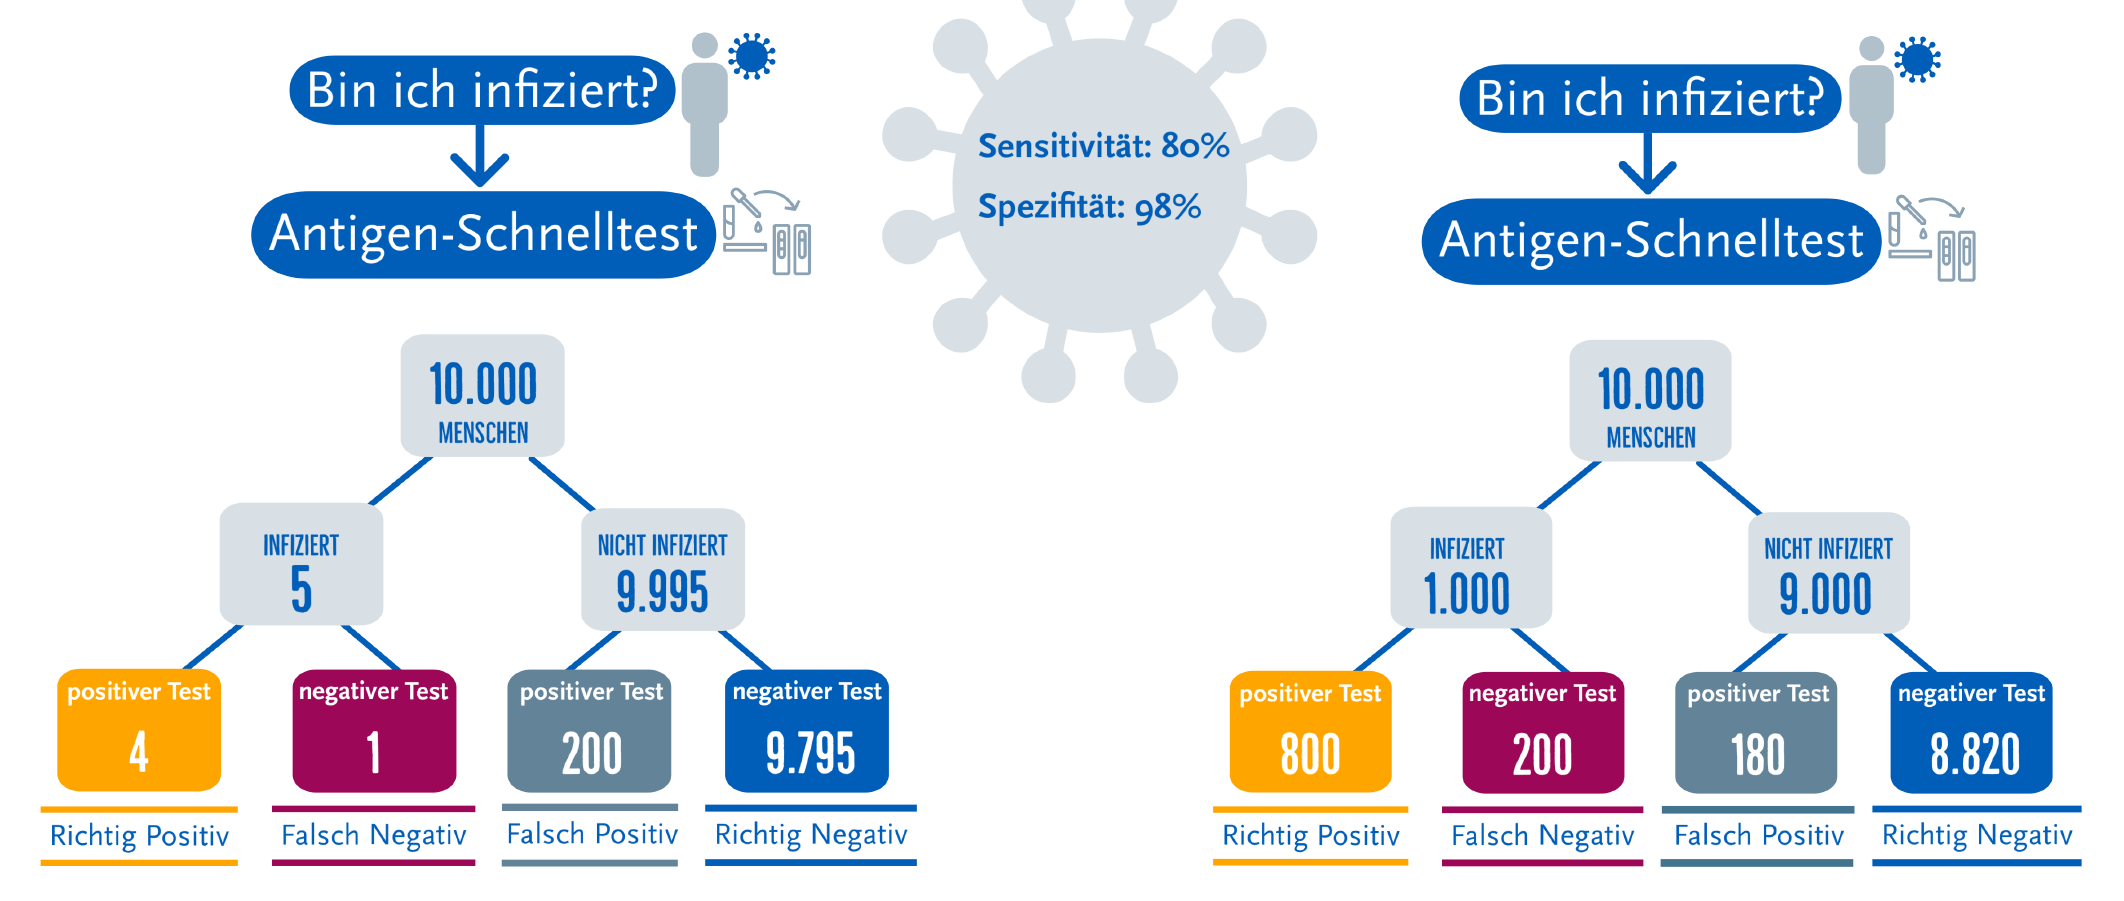
\includegraphics[width=\textwidth]{media/antigentest_rki.png}<5->
		\only<5->{\small Source: Robert Koch Institute}
		\note<5>{
			$5/10$k infected: $50\times$ higher probability of false-positive.
			This is a statistical reason why some tests are not done, if e.g. no symptoms are found.
		}
	\end{frame}

	\section{Bibliography}
	\begin{frame}{Bibliography}
		\centering
		\begin{thebibliography}{9}
			\bibitem{Lawrence} Lawrence A. (2019)
			\emph{Probability in Physics: An Introductory Guide},
			Springer Nature Switzerland, Chapters $1$ \& $7.1-7.5$,
			DOI~\href{https://doi.org/10.1007/978-3-030-04544-9}{10.1007/978-3-030-04544-9}

			\bibitem{GitBook}
				Clyde M. \emph{et al.} (2022)
				\emph{An Introduction to Bayesian Thinking: A Companion to the Statistics with R Course}, \href{https://statswithr.github.io/book/index.html}{Github.com/enstarprise},
				on 2022-06-15

			\bibitem{Bayes theorem}
				3Blue1Brown (2020) \emph{Bayes theorem, the geometry of changing beliefs},
			    \href{https://www.youtube.com/watch?v=HZGCoVF3YvM}{YouTube.com/watch?v=HZGCoVF3YvM},
				2024-11-16

			\bibitem{FrequentistTest}
                Kozyrkov C. (2020)
				\emph{Are you Bayesian or Frequentist?}
				\href{https://www.youtube.com/watch?v=GEFxFVESQXc}{YouTube.com/watch?v=GEFxFVESQXc},
				2024-11-16
		\end{thebibliography}
	\end{frame}

	\begin{frame}
		\centering
		\vspace{2cm}
		\textbf{\Huge \color{blue} Thank you for your attention!}
	\end{frame}
\end{document}